\documentclass{article}
\usepackage{amsmath}
\usepackage{amssymb}
\usepackage{tikz}
\usetikzlibrary{positioning}

\begin{document}

\begin{center}
    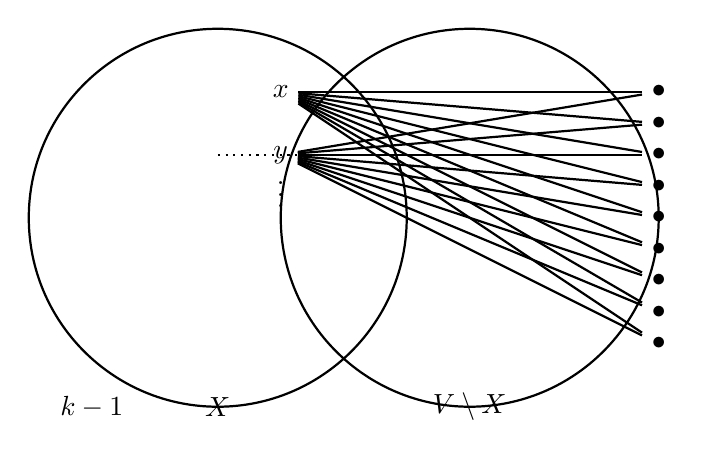
\begin{tikzpicture}[scale=0.8]
        % Define nodes
        \node (x) at (-1, 2) {$x$};
        \node (y) at (-1, 1) {$y$};
        \node (v1) at (5, 2) {$\bullet$};
        \node (v2) at (5, 1.5) {$\bullet$};
        \node (v3) at (5, 1) {$\bullet$};
        \node (v4) at (5, 0.5) {$\bullet$};
        \node (v5) at (5, 0) {$\bullet$};
        \node (v6) at (5, -0.5) {$\bullet$};
        \node (v7) at (5, -1) {$\bullet$};
        \node (v8) at (5, -1.5) {$\bullet$};
        \node (v9) at (5, -2) {$\bullet$};
        
        % Draw circles
        \draw[thick] (-2, 0) circle (3);
        \draw[thick] (2, 0) circle (3);
        
        % Draw edges
        \draw[thick] (x) -- (v1);
        \draw[thick] (x) -- (v2);
        \draw[thick] (x) -- (v3);
        \draw[thick] (x) -- (v4);
        \draw[thick] (x) -- (v5);
        \draw[thick] (x) -- (v6);
        \draw[thick] (x) -- (v7);
        \draw[thick] (x) -- (v8);
        \draw[thick] (x) -- (v9);
        
        \draw[thick] (y) -- (v1);
        \draw[thick] (y) -- (v2);
        \draw[thick] (y) -- (v3);
        \draw[thick] (y) -- (v4);
        \draw[thick] (y) -- (v5);
        \draw[thick] (y) -- (v6);
        \draw[thick] (y) -- (v7);
        \draw[thick] (y) -- (v8);
        \draw[thick] (y) -- (v9);
        
        % Draw dotted line
        \draw[dotted, thick] (-2, 1) -- (2, 1);
        
        % Labels
        \node at (-2, -3) {$X$};
        \node at (2, -3) {$V \setminus X$};
        \node at (-4, -3) {$k-1$};
        \node at (-1, 0.5) {$\vdots$};
    \end{tikzpicture}
\end{center}

Proof of Case 2 of \textbf{\autoref{Thm:cubic graph}} when $|N(\{x,y\})|=4$. The subgraph of $G$ induced by $X$ has a unique edge $xy$ and $e_G(X,V\setminus X)=3k+1$.

\end{document}